\let\negmedspace\undefined
\let\negthickspace\undefined
\documentclass[journal,12pt,twocolumn]{IEEEtran}
\usepackage{cite}
\usepackage{amsmath,amssymb,amsfonts,amsthm}
\usepackage{algorithmic}
\usepackage{graphicx}
\usepackage{textcomp}
\usepackage{xcolor}
\usepackage{txfonts}
\usepackage{listings}
\usepackage{enumitem}
\usepackage{mathtools}
\usepackage{gensymb}
\usepackage{comment}
\usepackage[breaklinks=true]{hyperref}
\usepackage{tkz-euclide} 
\usepackage{listings}
\usepackage{gvv}                                        
\def\inputGnumericTable{}                                 
\usepackage[latin1]{inputenc}                                
\usepackage{color}                                            
\usepackage{array}                                            
\usepackage{longtable}                                       
\usepackage{calc}                                             
\usepackage{multirow}                                         
\usepackage{hhline}                                           
\usepackage{ifthen}                                           
\usepackage{lscape}

\newtheorem{theorem}{Theorem}[section]
\newtheorem{problem}{Problem}
\newtheorem{proposition}{Proposition}[section]
\newtheorem{lemma}{Lemma}[section]
\newtheorem{corollary}[theorem]{Corollary}
\newtheorem{example}{Example}[section]
\newtheorem{definition}[problem]{Definition}
\newcommand{\BEQA}{\begin{eqnarray}}
\newcommand{\EEQA}{\end{eqnarray}}
\newcommand{\define}{\stackrel{\triangle}{=}}
\theoremstyle{remark}
\newtheorem{rem}{Remark}
\begin{document}

\bibliographystyle{IEEEtran}
\vspace{3cm}

\title{11.9.3.3}
\author{EE23BTECH11065 - prem sagar}
\maketitle
\newpage

\bigskip 

\renewcommand{\thefigure}{\theenumi}
\renewcommand{\thetable}{\theenumi}
\textbf{Question}:\\ The 5th,8th and 11th terms of a GP are p,q and s respectively .show that \[q^2=ps\]
\textbf{solution}:
\begin{align}
x(n)&= x(0)\,r^{n}, \text{if} n \geq 0
\\x(4)&=x(0)\,r^5
\\x(7)&=x(0)\,r^8
\\x({10})&=x(0)\,r^{11}
\\x(7)\,x(7)=x(0)\,r^8\,x(0)\,r^8
     \\ =x(0)^2\,r^{16}
\\x(4)\,x({10})=x(0)\,r^5\,x(0)\,r^{11}
       \\=x(0)^2\,r^{16}
\\x(7)^2=x(4)\,x({10})
\\q^2=ps
\end{align}
\begin{table}[!ht]
   \centering
        \begin{tabular}{|c|c|c|}
    \hline
            \textbf{Symbol} & \textbf{Value} & \textbf{Description} \\
    \hline
          $x(4)$ & $p$ & 5th term of G.P \\
    \hline
	  $x(7)$ & $q$ & 8th term of G.P\\
    \hline 
	  $x({10})$ &$s$ &11th term of G.P \\
    \hline
  \end{tabular}


    \caption{input parameters}
    \label{tab:11.9.3}
 \end{table}    
\\\begin{figure}
    \centering
    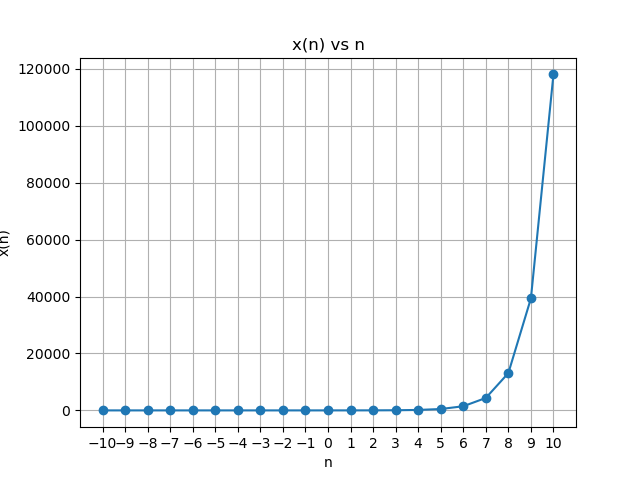
\includegraphics[width=1\linewidth]{/root/assign1/figs/figure__plot.png}
    \caption{plot x(n) vs n}
    \label{fig:enter-label}
\end{figure}\\
\\\begin{align}
\\x(n)\overset{Z}{\longleftrightarrow}   X(Z)
\\x(n)=x(0)\,r^n\,u(n)
\\X(Z)&=\sum_{n=-\infty}^{\infty}x(n) Z^{-n}\
     \\ &= \frac{x(0)}{1-r\,z^{-1}}\: \:,|z|>|r| \end{align}   
\end{document}
	
